\documentclass[11pt,a4paper]{article}

% =========================================================
%  PACKAGES
% =========================================================
\usepackage[utf8]{inputenc}
\usepackage[T1]{fontenc}
\usepackage{amsmath,amssymb,amsthm}
\usepackage{geometry}
\usepackage{xcolor}
\usepackage{tikz}
\usepackage{pgfplots}
\pgfplotsset{compat=1.18}
\usetikzlibrary{arrows.meta, positioning, shapes.geometric, calc, fit, backgrounds, decorations.pathreplacing, shadows}
\usepackage{booktabs}
\usepackage{enumitem}
\usepackage{hyperref}
\hypersetup{
    colorlinks=true,
    linkcolor=blue!50!black,
    urlcolor=blue!50!black,
    citecolor=blue!50!black,
    pdftitle={Retrieval-Augmented Generation: A Conceptual and Methodological Treatise},
    pdfauthor={AI Architecture \& NLP Systems Design}
}
\usepackage{fancyhdr}
\usepackage{titlesec}
\bibliographystyle{plain}

\geometry{margin=2.5cm}

% =========================================================
%  COLOR PALETTE
% =========================================================
\definecolor{ragblue}{RGB}{31,78,121}
\definecolor{raglight}{RGB}{214,234,248}
\definecolor{raggreen}{RGB}{39,116,79}
\definecolor{raglightgreen}{RGB}{212,239,223}
\definecolor{ragorange}{RGB}{202,111,30}
\definecolor{raglightorange}{RGB}{250,229,211}
\definecolor{ragpurple}{RGB}{93,64,140}
\definecolor{raglightpurple}{RGB}{229,222,242}
\definecolor{raggray}{RGB}{90,90,90}

\titleformat{\section}{\Large\bfseries\color{ragblue}}{\thesection}{1em}{}
\titleformat{\subsection}{\large\bfseries\color{ragblue!80!black}}{\thesubsection}{1em}{}
\titleformat{\subsubsection}{\normalsize\bfseries\color{raggray}}{\thesubsubsection}{1em}{}

\pagestyle{fancy}
\fancyhf{}
\fancyhead[L]{\small\textcolor{raggray}{Retrieval-Augmented Generation}}
\fancyhead[R]{\small\textcolor{raggray}{\thepage}}
\renewcommand{\headrulewidth}{0.4pt}

% =========================================================
%  TIKZ STYLES (reused across all diagrams)
% =========================================================
\tikzset{
  block/.style={
    rectangle, rounded corners=3pt, draw=ragblue, thick,
    fill=raglight, minimum width=6.4cm, minimum height=1.1cm,
    align=center, font=\small, drop shadow
  },
  ingestblock/.style={
    rectangle, rounded corners=3pt, draw=ragorange, thick,
    fill=raglightorange, minimum width=6.4cm, minimum height=1.1cm,
    align=center, font=\small, drop shadow
  },
  storeblock/.style={
    rectangle, rounded corners=3pt, draw=raggreen, thick,
    fill=raglightgreen, minimum width=6.4cm, minimum height=1.1cm,
    align=center, font=\small, drop shadow
  },
  genblock/.style={
    rectangle, rounded corners=3pt, draw=ragpurple, thick,
    fill=raglightpurple, minimum width=6.4cm, minimum height=1.1cm,
    align=center, font=\small, drop shadow
  },
  phase/.style={
    rectangle, draw=none, fill=none, font=\bfseries\small, text=raggray
  },
  arrowflow/.style={-{Latex[length=2.5mm]}, thick, draw=raggray},
  dataflow/.style={-{Latex[length=2mm]}, thick, dashed, draw=ragblue!70!black}
}

\newcommand{\sectionrule}{\vspace{-0.2cm}\noindent\textcolor{ragblue!40}{\rule{\linewidth}{0.6pt}}\vspace{0.3cm}}

% =========================================================
\title{
  \vspace{-1.5cm}
  {\color{ragblue}\Huge\bfseries Retrieval-Augmented Generation}\\[0.3cm]
  {\Large A Conceptual and Methodological Treatise on Grounded Language Model Architectures}
}
\author{AI Architecture \& Natural Language Processing Systems Design}
\date{\today}

% =========================================================
\begin{document}

\maketitle
\thispagestyle{empty}

\begin{abstract}
\noindent
Large Language Models (LLMs) are powerful statistical engines for language generation, yet they are fundamentally constrained by the boundaries of their training corpus: a fixed \emph{parametric memory} that is expensive to update, prone to factual drift, and incapable of reflecting information that did not exist at training time. \textbf{Retrieval-Augmented Generation (RAG)} is an architectural paradigm that addresses these constraints by coupling a generative model with a \emph{non-parametric}, externally queryable knowledge store. This document provides a rigorous, code-free, conceptual and methodological exploration of RAG systems, tracing the full lifecycle of data from raw ingestion, through chunking and vectorization, into indexed storage, and finally into retrieval-augmented synthesis. Mathematical formulations, architectural diagrams, and design trade-offs are presented throughout to build an end-to-end mental model suitable for both instructional and system-design purposes.
\end{abstract}

\vspace{0.5cm}
\tableofcontents
\newpage

% =========================================================
\section{High-Level Overview}
\sectionrule

\subsection{Defining Retrieval-Augmented Generation}

Retrieval-Augmented Generation (RAG) is a hybrid architecture, originally introduced by Lewis et al.~\cite{lewis2020rag}, that combines two previously distinct subfields of Natural Language Processing: \textbf{information retrieval (IR)} and \textbf{neural text generation}. Formally, a RAG system can be described as a conditional generation process in which the probability distribution over an output sequence $Y$ is conditioned not only on the input query $X$, but also on a set of retrieved evidentiary documents $\mathcal{D} = \{d_1, d_2, \dots, d_k\}$ sourced from an external corpus $\mathcal{C}$:

\begin{equation}
P(Y \mid X) \;=\; \sum_{\mathcal{D} \subseteq \mathcal{C}} P(\mathcal{D} \mid X) \cdot P(Y \mid X, \mathcal{D})
\end{equation}

In practice, the sum over all possible subsets of $\mathcal{C}$ is intractable, so RAG systems approximate this by \emph{deterministically} selecting the top-$k$ most relevant documents via a retriever $R$, and then conditioning generation on that fixed evidence set:

\begin{equation}
\mathcal{D}^{*} = R(X, \mathcal{C}, k), \qquad
P(Y \mid X) \;\approx\; P\big(Y \mid X, \mathcal{D}^{*}\big)
\end{equation}

This decomposition is the conceptual core of every RAG system: a \textbf{retriever} that narrows an enormous corpus down to a small, query-relevant evidence set, and a \textbf{generator} (the LLM) that synthesizes a coherent, grounded answer from that evidence.

\subsection{Why Standard LLMs Fall Short}

Standard, retrieval-free LLMs encode all of their ``knowledge'' inside their weight matrices during pretraining. This design has three structural weaknesses that RAG is explicitly built to overcome:

\begin{enumerate}[label=\textbf{(\alph*)}]
  \item \textbf{Hallucination.} Because an LLM generates tokens by sampling from a learned probability distribution rather than by consulting verified facts, it can produce fluent, syntactically confident statements that are factually incorrect. There is no internal mechanism forcing the model to ``check its work'' against a ground-truth source.
  \item \textbf{Static Knowledge Cutoff.} An LLM's parametric knowledge is frozen at the moment its pretraining corpus was assembled. Any event, publication, or fact that emerged after that point is structurally invisible to the model unless it is supplied at inference time.
  \item \textbf{Opacity and Non-Attributability.} Because knowledge in a parametric model is distributed across millions or billions of weights, it is not possible to point to the ``source'' of a given generated fact. This undermines trust, auditability, and compliance in high-stakes domains (legal, medical, financial).
\end{enumerate}

RAG mitigates all three weaknesses simultaneously: by grounding generation in explicitly retrieved passages, the model is far more likely to produce verifiable statements (reducing hallucination); by decoupling the knowledge store from the model weights, the corpus can be updated continuously without retraining (solving the static cutoff problem); and because every generated claim can be traced back to a retrieved chunk, the system gains \textbf{provenance} and \textbf{citability}.

\subsection{Scope: Naive RAG and Beyond}

The architecture described throughout this document corresponds to what the literature now terms \textbf{Naive RAG} (or \emph{standard RAG}): a linear pipeline of ingestion, vector indexing, top-$k$ semantic search, and single-pass generation. This is the foundational mental model, and it remains the starting point for nearly every production deployment.

However, the research community has rapidly extended this baseline into more sophisticated paradigms that address specific failure modes of the naive approach. For completeness, we note the principal SOTA extensions without developing them in detail:

\begin{description}
  \item[Self-RAG.] Introduces reflection tokens that allow the LLM to \emph{self-evaluate} whether retrieval is needed, whether retrieved passages are relevant, and whether the generated output is supported by the evidence---enabling adaptive retrieval and built-in factuality checks~\cite{asai2023selfrag}.
  \item[GraphRAG.] Replaces or augments flat vector stores with knowledge graphs, capturing relational structure (entities, edges, communities) that enables multi-hop reasoning and global summarization over interconnected facts~\cite{zhang2025graphrag}.
  \item[Multimodal RAG.] Extends the ingestion and retrieval pipeline beyond text to include images, tables, audio, and video, using cross-modal embedding spaces or modality-specific extractors to ground generation in non-textual evidence~\cite{mei2025multimodal}.
\end{description}

These paradigms are not mutually exclusive; modern production systems frequently combine elements from several (e.g., GraphRAG with self-reflective retrieval). The reader seeking a comprehensive taxonomy of RAG system variants is referred to the survey by Sharma~\cite{sharma2025rag}.

\subsection{The Three-Phase Mental Model}

Throughout this document, RAG is decomposed into three sequential phases, which together form a pipeline that transforms raw, unstructured data into a grounded, natural-language answer:

\begin{center}
\begin{tabular}{@{}lll@{}}
\toprule
\textbf{Phase} & \textbf{Name} & \textbf{Core Question Answered} \\
\midrule
1 & Ingestion Pipeline & ``How do we turn raw documents into searchable units?'' \\
2 & Storage \& Retrieval & ``How do we find the most relevant units for a query?'' \\
3 & Prompt Injection \& Generation & ``How do we turn evidence into a grounded answer?'' \\
\bottomrule
\end{tabular}
\end{center}

Figure~\ref{fig:master-pipeline} presents the master architectural diagram that governs the remainder of this document; each subsequent section elaborates on one segment of this pipeline.

\begin{figure}[htbp]
\centering
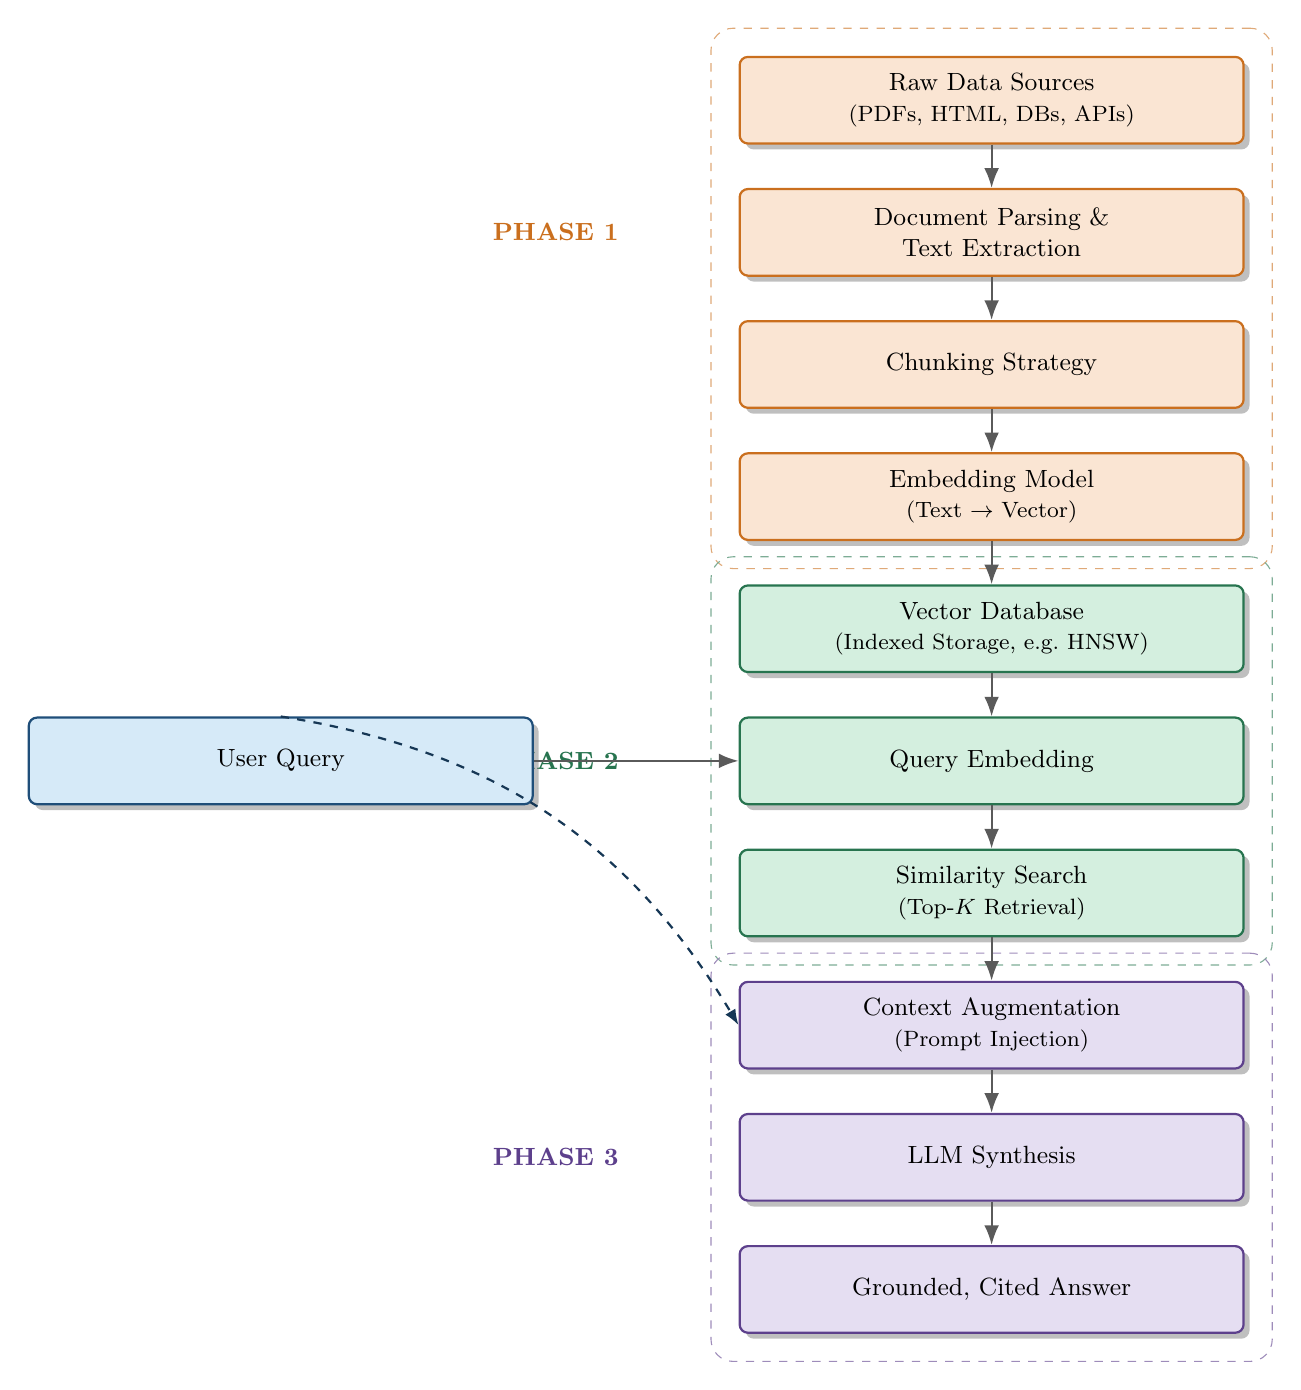
\begin{tikzpicture}[node distance=0.55cm]

% Phase 1 group
\node[ingestblock] (raw) {Raw Data Sources\\ \footnotesize (PDFs, HTML, DBs, APIs)};
\node[ingestblock, below=of raw] (parse) {Document Parsing \& \\Text Extraction};
\node[ingestblock, below=of parse] (chunk) {Chunking Strategy};
\node[ingestblock, below=of chunk] (embed) {Embedding Model \\ \footnotesize (Text $\rightarrow$ Vector)};

% Phase 2 group
\node[storeblock, below=of embed] (store) {Vector Database \\ \footnotesize (Indexed Storage, e.g.\ HNSW)};
\node[storeblock, below=of store] (query) {Query Embedding};
\node[storeblock, below=of query] (search) {Similarity Search \\ \footnotesize (Top-$K$ Retrieval)};

% Phase 3 group
\node[genblock, below=of search] (inject) {Context Augmentation \\ \footnotesize (Prompt Injection)};
\node[genblock, below=of inject] (llm) {LLM Synthesis};
\node[genblock, below=of llm] (answer) {Grounded, Cited Answer};

% Arrows
\foreach \a/\b in {raw/parse, parse/chunk, chunk/embed, embed/store, store/query, query/search, search/inject, inject/llm, llm/answer}
  \draw[arrowflow] (\a) -- (\b);

% Phase labels on the side
\node[phase, left=1.4cm of parse, text=ragorange] {PHASE 1};
\node[phase, left=1.4cm of query, text=raggreen] {PHASE 2};
\node[phase, left=1.4cm of llm, text=ragpurple] {PHASE 3};

% Background groupings
\begin{scope}[on background layer]
\node[fit=(raw)(embed), inner sep=0.35cm, rounded corners=8pt, draw=ragorange!60, dashed] {};
\node[fit=(store)(search), inner sep=0.35cm, rounded corners=8pt, draw=raggreen!60, dashed] {};
\node[fit=(inject)(answer), inner sep=0.35cm, rounded corners=8pt, draw=ragpurple!60, dashed] {};
\end{scope}

% User query entry point
\node[block, left=2.6cm of query, fill=raglight] (userq) {User Query};
\draw[arrowflow] (userq) -- (query);
\draw[dataflow] (userq.north) to[bend left=25] (inject.west);

\end{tikzpicture}
\caption{Master end-to-end RAG data flow: from raw data ingestion, through vectorized storage and similarity-based retrieval, to prompt injection and final grounded generation. The dashed blue arrow indicates that the original user query is also passed forward into the final prompt alongside the retrieved context.}
\label{fig:master-pipeline}
\end{figure}

\newpage

% =========================================================
\section{Phase 1: The Ingestion Pipeline}
\sectionrule

The ingestion pipeline is the offline (or periodically refreshed) process by which an organization's raw, heterogeneous data is transformed into a structured, searchable knowledge base. It is arguably the phase where the majority of real-world RAG system quality is won or lost: poor parsing or naive chunking propagates errors through every downstream stage.

\subsection{Document Parsing and Text Extraction}

Raw enterprise or web data rarely arrives as clean plain text. It typically exists as PDFs, HTML pages, Word documents, spreadsheets, scanned images, presentation slides, or structured records from relational databases and APIs. The \textbf{parsing} stage is responsible for normalizing all of these heterogeneous formats into a canonical textual representation while preserving as much semantically useful structure as possible.

Key conceptual concerns at this stage include:

\begin{itemize}
  \item \textbf{Structural Preservation.} Headings, tables, bullet lists, and section boundaries carry meaning. A naive parser that flattens a PDF into an unstructured character stream destroys this signal, whereas a structure-aware parser can preserve hierarchy (e.g., tagging a paragraph as belonging to ``Section 3.2'').
  \item \textbf{Noise Removal.} Headers, footers, page numbers, watermarks, and boilerplate navigation menus (in HTML) constitute noise that, if left in place, pollutes the embedding space with irrelevant repeated tokens.
  \item \textbf{Multi-Modal Extraction.} Tables, charts, and embedded images often carry information not present in surrounding prose. Conceptually, these require specialized extraction routines (e.g., table-structure recognition) so that tabular relationships are not lost when flattened to text.
  \item \textbf{Metadata Capture.} Provenance data --- source filename, page number, author, timestamp, section title --- must be captured and carried forward. This metadata becomes essential later for filtering, citation, and re-ranking.
\end{itemize}

The output of this stage is a set of \emph{normalized documents}: clean text, annotated with structural and provenance metadata, ready to be subdivided.

\subsection{File Chunking}

A single source document is almost always too large to serve as a single retrieval unit: it may be thousands or tens of thousands of tokens long, while embedding models and LLM context windows operate efficiently over much smaller spans. \textbf{Chunking} is the process of subdividing normalized documents into smaller, semantically coherent units that will each be independently embedded and indexed.

\subsubsection{Why Chunking Is Crucial}

Chunking strategy directly determines retrieval quality along two competing axes:

\begin{itemize}
  \item \textbf{Precision:} Smaller chunks yield embeddings that are more topically concentrated, meaning retrieval is less likely to return a chunk that is only tangentially related to the query.
  \item \textbf{Context Sufficiency:} Chunks that are too small may fragment an idea across multiple chunks, causing the retriever to return a piece of an argument without the surrounding context needed to correctly interpret it.
\end{itemize}

This trade-off is often termed the \textbf{granularity dilemma}, and no single chunk size is optimal across all corpora; instead, practitioners choose a strategy suited to the structure of their data.

\subsubsection{Chunking Strategies}

\begin{description}
  \item[Fixed-Size Chunking.] The simplest strategy: text is split every $n$ tokens (or characters), regardless of sentence or paragraph boundaries. It is computationally trivial and produces highly predictable chunk sizes, but it risks severing sentences or ideas mid-thought.
  \item[Sliding Window Chunking (with Overlap).] A refinement of fixed-size chunking in which consecutive chunks share an overlapping region of $o$ tokens. If chunk $i$ spans tokens $[t_i, t_i + n]$, then chunk $i+1$ begins at $t_{i+1} = t_i + (n - o)$ rather than at $t_i + n$. This overlap ensures that an idea straddling a chunk boundary is still fully captured within at least one chunk, at the cost of some storage redundancy.
  \item[Semantic Chunking.] Rather than splitting at a fixed token count, boundaries are placed at points of maximal topical discontinuity --- for instance, by measuring the embedding-space distance between consecutive sentences and inserting a boundary wherever that distance exceeds a threshold. This produces variable-length chunks that are more likely to represent a single coherent idea.
  \item[Structure-Aware (Recursive) Chunking.] Splitting is guided by the document's own structural hierarchy --- first attempting to split along section or heading boundaries, then paragraphs, then sentences, only falling back to a hard token cut when a structural unit is still too large. This respects the author's own organization of ideas.
\end{description}

Figure~\ref{fig:chunking} illustrates these strategies conceptually.

\begin{figure}[htbp]
\centering
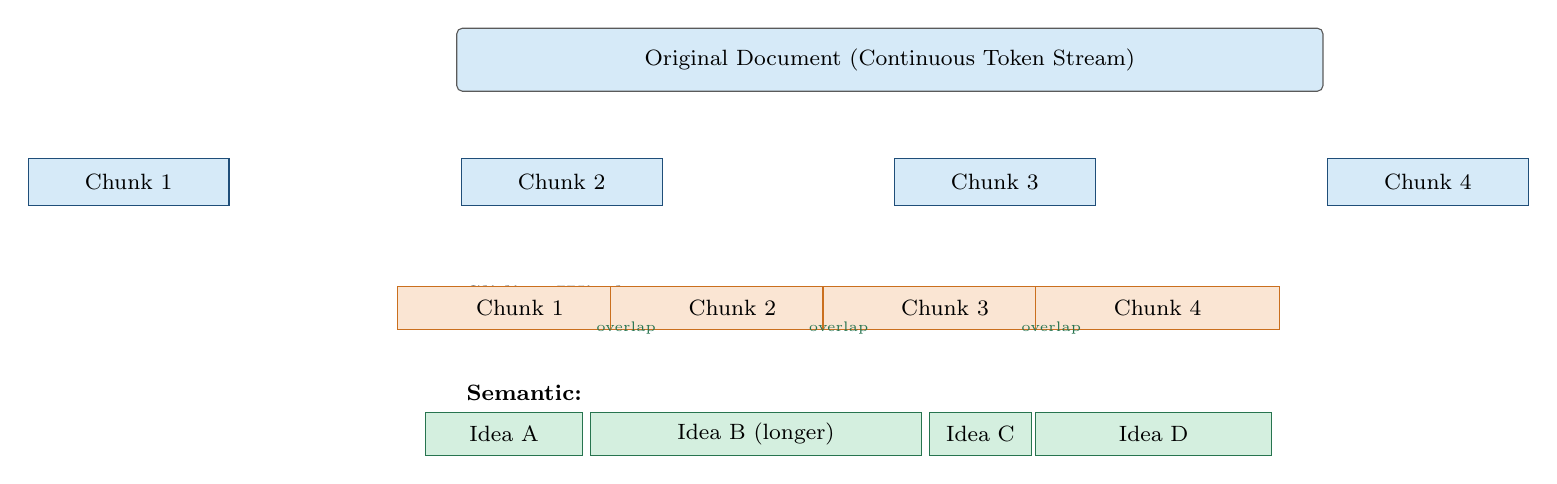
\begin{tikzpicture}[node distance=0.4cm, font=\footnotesize]

% Original document bar
\node[draw=raggray, fill=raglight, minimum width=11cm, minimum height=0.8cm, rounded corners=2pt] (doc) {Original Document (Continuous Token Stream)};

% Fixed-size chunking
\node[below=1.1cm of doc, anchor=north west, xshift=-5.5cm] (lab1) {\textbf{Fixed-Size:}};
\foreach \i/\x in {1/-5.5,2/-2.75,3/0,4/2.75}
  \node[draw=ragblue, fill=raglight, minimum width=2.55cm, minimum height=0.6cm, right=0.05cm of lab1, xshift=\x cm] at (\x,-1.55) {Chunk \i};

% Sliding window with overlap
\node[below=2.35cm of doc, anchor=north west, xshift=-5.5cm] (lab2) {\textbf{Sliding Window:}};
\node[draw=ragorange, fill=raglightorange, minimum width=3.1cm, minimum height=0.55cm] at (-4.7,-3.15) {Chunk 1};
\node[draw=ragorange, fill=raglightorange, minimum width=3.1cm, minimum height=0.55cm] at (-2.0,-3.15) {Chunk 2};
\node[draw=ragorange, fill=raglightorange, minimum width=3.1cm, minimum height=0.55cm] at (0.7,-3.15) {Chunk 3};
\node[draw=ragorange, fill=raglightorange, minimum width=3.1cm, minimum height=0.55cm] at (3.4,-3.15) {Chunk 4};
\node[font=\tiny, text=raggreen, below=0.05cm] at (-3.35,-3.15) {overlap};
\node[font=\tiny, text=raggreen, below=0.05cm] at (-0.65,-3.15) {overlap};
\node[font=\tiny, text=raggreen, below=0.05cm] at (2.05,-3.15) {overlap};

% Semantic chunking
\node[below=3.6cm of doc, anchor=north west, xshift=-5.5cm] (lab3) {\textbf{Semantic:}};
\node[draw=raggreen, fill=raglightgreen, minimum width=2.0cm, minimum height=0.55cm] at (-4.9,-4.75) {Idea A};
\node[draw=raggreen, fill=raglightgreen, minimum width=4.2cm, minimum height=0.55cm] at (-1.7,-4.75) {Idea B (longer)};
\node[draw=raggreen, fill=raglightgreen, minimum width=1.3cm, minimum height=0.55cm] at (1.15,-4.75) {Idea C};
\node[draw=raggreen, fill=raglightgreen, minimum width=3.0cm, minimum height=0.55cm] at (3.35,-4.75) {Idea D};

\end{tikzpicture}
\caption{Conceptual comparison of chunking strategies applied to the same source document: fixed-size chunking ignores content boundaries; sliding-window chunking introduces deliberate overlap between adjacent chunks; semantic chunking produces variable-length chunks aligned to topical boundaries.}
\label{fig:chunking}
\end{figure}

\subsection{Vector Embeddings}

Once chunks are produced, each chunk of text must be transformed into a form that a computer can compare mathematically for \emph{semantic} similarity, rather than mere keyword overlap. This transformation is performed by an \textbf{embedding model}.

\subsubsection{Conceptual Definition}

An embedding model is a neural network, typically a Transformer-based encoder, trained (often via contrastive learning objectives) so that texts with similar meaning are mapped to nearby points in a high-dimensional continuous vector space, while texts with dissimilar meaning are mapped to distant points. Formally, an embedding function $E$ maps a chunk of text $c$ to a dense vector:

\begin{equation}
E: \text{Text} \longrightarrow \mathbb{R}^{d}, \qquad \mathbf{v}_c = E(c)
\end{equation}

where $d$ is the fixed dimensionality of the embedding space (commonly ranging from a few hundred to a few thousand dimensions, depending on the model).

\subsubsection{Why Dense Vectors Capture Meaning}

Unlike sparse, keyword-based representations (e.g., bag-of-words or TF-IDF vectors, where dimensions correspond to literal vocabulary terms), dense embeddings distribute meaning across all dimensions simultaneously. Because the encoder is trained on massive corpora to predict contextual relationships between words and sentences, the resulting vector space exhibits an emergent property: \textbf{semantic proximity mirrors geometric proximity}. Two sentences that express the same idea using entirely different vocabulary (e.g., ``the feline sat on the rug'' and ``a cat rested on the carpet'') will be encoded to vectors that are close together in $\mathbb{R}^d$, even though they share almost no literal tokens. This is the property that ultimately allows RAG systems to perform \emph{meaning-based} retrieval rather than brittle keyword matching.

\begin{figure}[htbp]
\centering
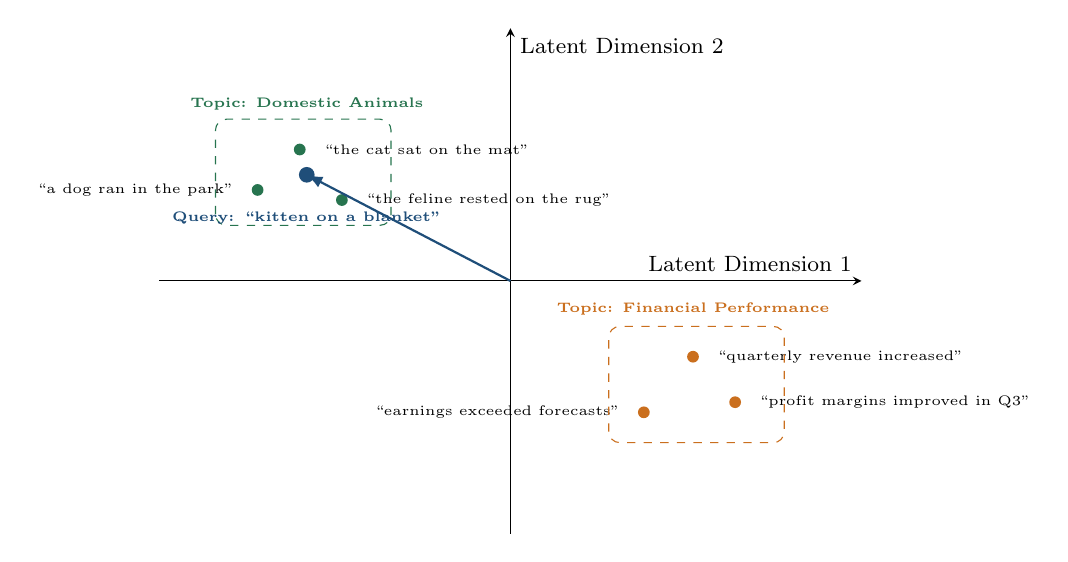
\begin{tikzpicture}[font=\footnotesize]
\begin{axis}[
  width=10.5cm, height=8cm,
  xlabel={Latent Dimension 1}, ylabel={Latent Dimension 2},
  axis lines=middle,
  xmin=-5, xmax=5, ymin=-5, ymax=5,
  xtick=\empty, ytick=\empty,
  clip=false
]
% Cluster A - animals
\node[circle, fill=raggreen, inner sep=1.5pt] at (axis cs:-3,2.6) {};
\node[anchor=west, font=\tiny] at (axis cs:-2.8,2.6) {``the cat sat on the mat''};
\node[circle, fill=raggreen, inner sep=1.5pt] at (axis cs:-3.6,1.8) {};
\node[anchor=east, font=\tiny] at (axis cs:-3.8,1.8) {``a dog ran in the park''};
\node[circle, fill=raggreen, inner sep=1.5pt] at (axis cs:-2.4,1.6) {};
\node[anchor=west, font=\tiny] at (axis cs:-2.2,1.6) {``the feline rested on the rug''};
\draw[dashed, raggreen, rounded corners] (axis cs:-4.2,1.1) rectangle (axis cs:-1.7,3.2);
\node[raggreen, font=\bfseries\tiny] at (axis cs:-2.9,3.5) {Topic: Domestic Animals};

% Cluster B - finance
\node[circle, fill=ragorange, inner sep=1.5pt] at (axis cs:2.6,-1.5) {};
\node[anchor=west, font=\tiny] at (axis cs:2.8,-1.5) {``quarterly revenue increased''};
\node[circle, fill=ragorange, inner sep=1.5pt] at (axis cs:3.2,-2.4) {};
\node[anchor=west, font=\tiny] at (axis cs:3.4,-2.4) {``profit margins improved in Q3''};
\node[circle, fill=ragorange, inner sep=1.5pt] at (axis cs:1.9,-2.6) {};
\node[anchor=east, font=\tiny] at (axis cs:1.7,-2.6) {``earnings exceeded forecasts''};
\draw[dashed, ragorange, rounded corners] (axis cs:1.4,-3.2) rectangle (axis cs:3.9,-0.9);
\node[ragorange, font=\bfseries\tiny] at (axis cs:2.6,-0.55) {Topic: Financial Performance};

% Query vector
\node[circle, fill=ragblue, inner sep=2pt] at (axis cs:-2.9,2.1) {};
\node[ragblue, font=\bfseries\tiny, anchor=north] at (axis cs:-2.9,1.55) {Query: ``kitten on a blanket''};
\draw[-{Latex[length=2mm]}, ragblue, thick] (axis cs:0,0) -- (axis cs:-2.9,2.1);
\end{axis}
\end{tikzpicture}
\caption{A conceptual 2-D projection of a high-dimensional embedding space. Semantically related sentences cluster together regardless of exact vocabulary overlap; a new query vector lands nearest to the semantically relevant cluster, enabling meaning-based retrieval.}
\label{fig:embedding-space}
\end{figure}

\newpage

% =========================================================
\section{Phase 2: Storage \& Retrieval}
\sectionrule

Once every chunk has been converted into a vector, the system must store these vectors in a way that allows extremely fast similarity search over potentially millions or billions of entries. This is the responsibility of the \textbf{vector database}.

\subsection{Vector Databases and Indexing}

A vector database is a specialized data store optimized for a single fundamental operation: given a query vector, efficiently return the $k$ stored vectors that are closest to it under a chosen distance metric. This operation is known as \textbf{Approximate Nearest Neighbor (ANN) search}.

\subsubsection{Why ``Approximate'' Nearest Neighbor}

An exact nearest-neighbor search requires computing the distance between the query vector and every single stored vector --- an $O(N \cdot d)$ operation for $N$ stored vectors of dimension $d$. At web scale, where $N$ can be in the hundreds of millions, this brute-force approach is computationally prohibitive for real-time applications. ANN algorithms trade a small, controllable amount of recall (i.e., they may occasionally miss the true nearest neighbor) for orders-of-magnitude improvements in query latency, typically achieving sub-linear or even logarithmic search complexity.

\subsubsection{Hierarchical Navigable Small World (HNSW)}

One of the most widely used indexing structures in modern vector databases is \textbf{HNSW}. Conceptually, HNSW builds a multi-layered graph structure over the set of stored vectors:

\begin{itemize}
  \item Each vector is a \textbf{node} in the graph, connected to a small number of ``nearby'' nodes (its approximate neighbors).
  \item The graph is organized into multiple \textbf{layers}, where the top layer contains only a sparse subset of nodes with long-range connections (enabling large jumps across the vector space), and each successive lower layer contains progressively more nodes with shorter, denser connections.
  \item A search begins at an entry point in the topmost (sparsest) layer and greedily traverses to the neighbor closest to the query vector, then ``drops down'' a layer and repeats, refining the search at each level until it reaches the bottom (densest) layer, where a fine-grained neighborhood search yields the final candidate set.
\end{itemize}

This layered structure is analogous to a highway system: the top layer represents interstate highways that quickly move the search into the right general region, while lower layers represent progressively smaller local roads that pinpoint the exact destination.

\begin{figure}[htbp]
\centering
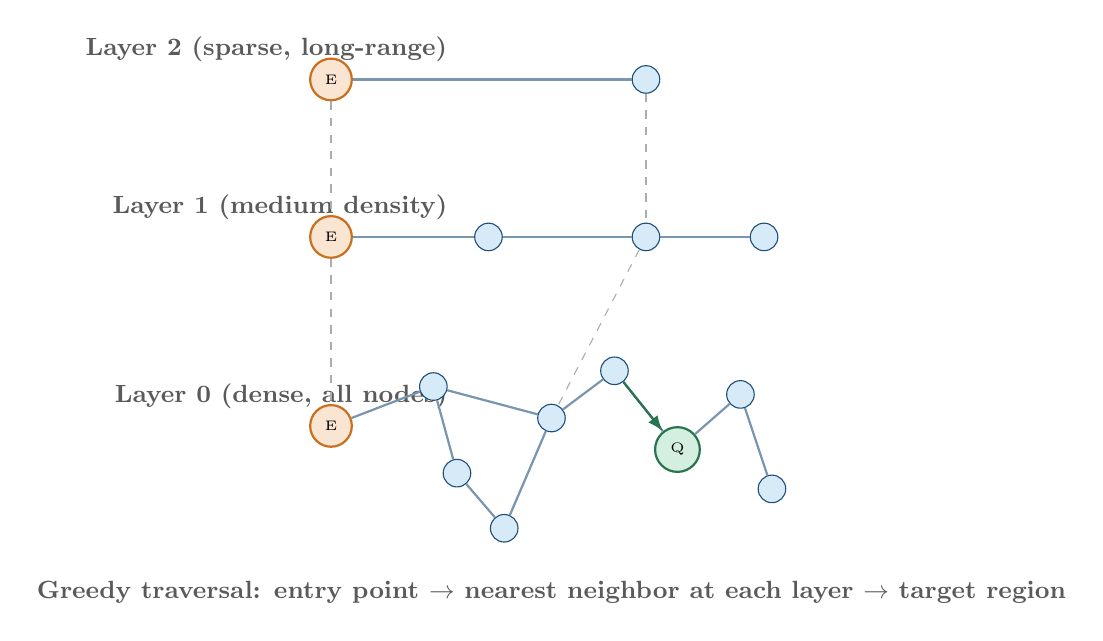
\begin{tikzpicture}[
  node/.style={circle, draw=ragblue, fill=raglight, minimum size=0.35cm, font=\tiny},
  entrynode/.style={circle, draw=ragorange, fill=raglightorange, minimum size=0.4cm, font=\tiny, thick},
  targetnode/.style={circle, draw=raggreen, fill=raglightgreen, minimum size=0.4cm, font=\tiny, thick}
]

% Layer 2 (top, sparse)
\node[phase, above left=0.1cm and -1.6cm of {(0,6)}] {Layer 2 (sparse, long-range)};
\node[entrynode] (l2a) at (0,6) {E};
\node[node] (l2b) at (4,6) {};
\draw[thick, ragblue!60] (l2a) -- (l2b);

% Layer 1 (middle)
\node[phase, above left=0.1cm and -1.6cm of {(0,4)}] {Layer 1 (medium density)};
\node[entrynode] (l1a) at (0,4) {E};
\node[node] (l1b) at (2,4) {};
\node[node] (l1c) at (4,4) {};
\node[node] (l1d) at (5.5,4) {};
\draw[thick, ragblue!60] (l1a) -- (l1b) -- (l1c) -- (l1d);
\draw[dashed, raggray!50] (l2a) -- (l1a);
\draw[dashed, raggray!50] (l2b) -- (l1c);

% Layer 0 (bottom, dense - full graph)
\node[phase, above left=0.1cm and -1.6cm of {(0,1.6)}] {Layer 0 (dense, all nodes)};
\node[entrynode] (l0a) at (0,1.6) {E};
\node[node] (l0b) at (1.3,2.1) {};
\node[node] (l0c) at (1.6,1.0) {};
\node[node] (l0d) at (2.8,1.7) {};
\node[node] (l0e) at (3.6,2.3) {};
\node[targetnode] (l0f) at (4.4,1.3) {Q};
\node[node] (l0g) at (5.2,2.0) {};
\node[node] (l0h) at (5.6,0.8) {};
\node[node] (l0i) at (2.2,0.3) {};

\draw[thick, ragblue!60] (l0a) -- (l0b) -- (l0d) -- (l0e) -- (l0f);
\draw[thick, ragblue!60] (l0b) -- (l0c) -- (l0i) -- (l0d);
\draw[thick, ragblue!60] (l0f) -- (l0g) -- (l0h);
\draw[thick, raggreen, {-Latex[length=2mm]}] (l0e) -- (l0f);

\draw[dashed, raggray!50] (l1a) -- (l0a);
\draw[dashed, raggray!50] (l1c) -- (l0d);

\node[phase, below=0.15cm of {(2.8,-0.1)}, text=raggray] {Greedy traversal: entry point $\to$ nearest neighbor at each layer $\to$ target region};

\end{tikzpicture}
\caption{Conceptual illustration of HNSW multi-layer graph traversal. The search enters at a sparse top layer (fast, long-range jumps) and descends through progressively denser layers, greedily following edges toward the query vector \textbf{Q} until the closest node in the bottom, fully-connected layer is located.}
\label{fig:hnsw}
\end{figure}

\subsection{Similarity Metrics}

Given a query vector $\mathbf{q} \in \mathbb{R}^d$ and a candidate stored vector $\mathbf{v} \in \mathbb{R}^d$, a \textbf{similarity metric} (or its inverse, a distance metric) quantifies how ``close'' the two vectors are in the embedding space. The three most common metrics used in vector retrieval are:

\subsubsection{Cosine Similarity}

Cosine similarity measures the cosine of the angle between two vectors, ignoring their magnitude entirely and focusing purely on direction:

\begin{equation}
\text{cos\_sim}(\mathbf{q}, \mathbf{v}) = \frac{\mathbf{q} \cdot \mathbf{v}}{\lVert \mathbf{q} \rVert \, \lVert \mathbf{v} \rVert} = \frac{\sum_{i=1}^{d} q_i v_i}{\sqrt{\sum_{i=1}^{d} q_i^2}\sqrt{\sum_{i=1}^{d} v_i^2}}
\end{equation}

The result ranges from $-1$ (perfectly opposite) to $1$ (perfectly aligned), with $0$ indicating orthogonality (no relationship). Because it is magnitude-invariant, cosine similarity is particularly well suited to text embeddings, where vector magnitude often reflects incidental factors such as text length rather than semantic content.

\subsubsection{Dot Product}

The dot product (or inner product) is the un-normalized counterpart to cosine similarity:

\begin{equation}
\text{dot}(\mathbf{q}, \mathbf{v}) = \mathbf{q} \cdot \mathbf{v} = \sum_{i=1}^{d} q_i v_i
\end{equation}

Unlike cosine similarity, the dot product is sensitive to vector magnitude, meaning that longer or more ``confident'' vectors can score higher independent of directional alignment. When embeddings are pre-normalized to unit length (i.e., $\lVert \mathbf{v} \rVert = 1$), the dot product becomes mathematically equivalent to cosine similarity, which is why many production systems normalize vectors at indexing time and then use the computationally cheaper dot product at query time.

\subsubsection{Euclidean (L2) Distance}

Euclidean distance measures the straight-line geometric distance between two points in the vector space:

\begin{equation}
\text{L2}(\mathbf{q}, \mathbf{v}) = \lVert \mathbf{q} - \mathbf{v} \rVert_2 = \sqrt{\sum_{i=1}^{d} (q_i - v_i)^2}
\end{equation}

Unlike the previous two metrics, this is a \emph{distance} rather than a \emph{similarity}: smaller values indicate closer, more similar vectors. Euclidean distance is sensitive to both the direction and magnitude of the difference between vectors, and is most appropriate when the absolute geometric position of embeddings (not merely their orientation) is meaningful for the embedding model in use.

\begin{center}
\begin{tabular}{@{}p{3.2cm}p{5.4cm}p{5.8cm}@{}}
\toprule
\textbf{Metric} & \textbf{Sensitivity} & \textbf{Typical Use Case} \\
\midrule
Cosine Similarity & Direction only (magnitude-invariant) & General-purpose text similarity; most common default \\
Dot Product & Direction \emph{and} magnitude & Pre-normalized embeddings; maximum-inner-product search \\
Euclidean (L2) & Absolute geometric distance & Embedding spaces where magnitude carries semantic weight \\
\bottomrule
\end{tabular}
\end{center}

\subsection{Similarity Search: Query Vectorization and Top-\texorpdfstring{$K$}{K} Retrieval}

At query time, the retrieval process mirrors the ingestion process in miniature: the user's natural-language query $X$ is passed through the \emph{same} embedding model $E$ used during ingestion, producing a query vector $\mathbf{q} = E(X)$. This vector is then submitted to the vector database's ANN index, which returns the $k$ stored chunk-vectors with the highest similarity (or lowest distance) score:

\begin{equation}
\mathcal{D}^{*} = \operatorname*{arg\,top\text{-}k}_{v \,\in\, \mathcal{C}_{\text{vec}}} \; \text{sim}(\mathbf{q}, v)
\end{equation}

The choice of $k$ is itself a design decision: too small a $k$ risks omitting a necessary piece of evidence, while too large a $k$ dilutes the eventual prompt with marginally relevant or redundant chunks and consumes valuable context-window budget. Production systems frequently apply a secondary \textbf{re-ranking} stage --- a more computationally expensive but more accurate relevance model applied only to the small candidate set returned by the ANN search --- to refine the final ordering before the top chunks are passed forward.

\begin{figure}[htbp]
\centering
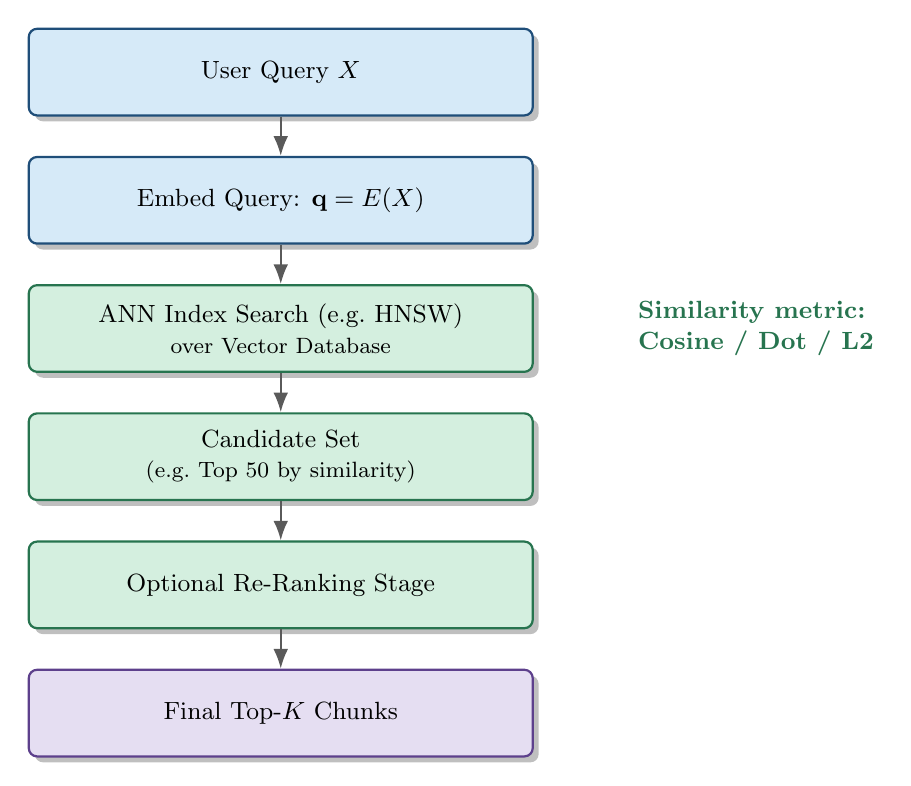
\begin{tikzpicture}[node distance=0.5cm]

\node[block] (q) {User Query $X$};
\node[block, below=of q] (embedq) {Embed Query: $\mathbf{q} = E(X)$};
\node[storeblock, below=of embedq] (index) {ANN Index Search (e.g.\ HNSW) \\ \footnotesize over Vector Database};
\node[storeblock, below=of index] (candidates) {Candidate Set \\ \footnotesize (e.g.\ Top 50 by similarity)};
\node[storeblock, below=of candidates] (rerank) {Optional Re-Ranking Stage};
\node[genblock, below=of rerank] (topk) {Final Top-$K$ Chunks};

\foreach \a/\b in {q/embedq, embedq/index, index/candidates, candidates/rerank, rerank/topk}
  \draw[arrowflow] (\a) -- (\b);

\node[phase, right=1.2cm of index, text=raggreen, align=left] {Similarity metric:\\ Cosine / Dot / L2};
\end{tikzpicture}
\caption{The similarity search sub-pipeline: the query is embedded with the same model used for the corpus, an approximate nearest-neighbor search returns an initial candidate set, and an optional re-ranking stage refines the final Top-$K$ chunks passed to generation.}
\label{fig:similarity-search}
\end{figure}

\newpage

% =========================================================
\section{Phase 3: Prompt Injection \& Generation}
\sectionrule

The final phase transforms retrieved evidence into a natural-language response. This is where the retrieval subsystem and the generative LLM are architecturally fused.

\subsection{Context Augmentation}

\textbf{Context augmentation} (also called prompt injection or prompt assembly, not to be confused with the security vulnerability of the same name) is the process of constructing the final prompt that will be sent to the LLM. Conceptually, this prompt is assembled from three components:

\begin{enumerate}
  \item \textbf{System Instructions.} A directive establishing the model's role and behavioral constraints --- for example, instructing the model to answer strictly using the provided context, to cite sources, and to explicitly state when the retrieved context does not contain sufficient information to answer.
  \item \textbf{Retrieved Context.} The Top-$K$ chunks returned by the retrieval stage, typically concatenated together, often with their provenance metadata (source document, section, page) interleaved so the model can generate accurate citations.
  \item \textbf{The Original User Query.} The user's original natural-language question, placed so the model understands precisely what it must answer using the supplied context.
  \end{enumerate}

The ordering and formatting of these components matters conceptually: placing the most relevant chunk closer to the query, clearly delimiting chunk boundaries (so the model does not conflate two distinct sources), and explicitly instructing the model on how to behave when evidence is insufficient are all design levers that materially affect answer quality and faithfulness.

\subsection{LLM Synthesis}

Once the augmented prompt is assembled, it is passed to the generative LLM, which performs \textbf{synthesis}: producing a final natural-language answer conditioned jointly on the user's query and the retrieved evidence, as originally formalized in Equation~(2). Conceptually, synthesis involves several implicit sub-tasks that the LLM performs simultaneously during generation:

\begin{itemize}
  \item \textbf{Relevance Filtering.} Even within the Top-$K$ retrieved chunks, not every sentence is necessarily useful; the model must implicitly identify which portions of the context are actually responsive to the query.
  \item \textbf{Cross-Chunk Synthesis.} When the answer requires combining information from multiple retrieved chunks (e.g., reconciling a definition from one source with a statistic from another), the model must perform reasoning \emph{across} the provided evidence rather than merely extracting a single passage verbatim.
  \item \textbf{Faithfulness / Groundedness.} A well-instructed RAG system should generate an answer that is \emph{entailed} by the retrieved context, rather than reverting to unsupported parametric knowledge --- this is the central mechanism by which RAG suppresses hallucination.
  \item \textbf{Abstention.} When the retrieved context does not sufficiently answer the query, a well-designed system should explicitly communicate this rather than fabricating a plausible-sounding but ungrounded answer.
\end{itemize}

\begin{figure}[htbp]
\centering
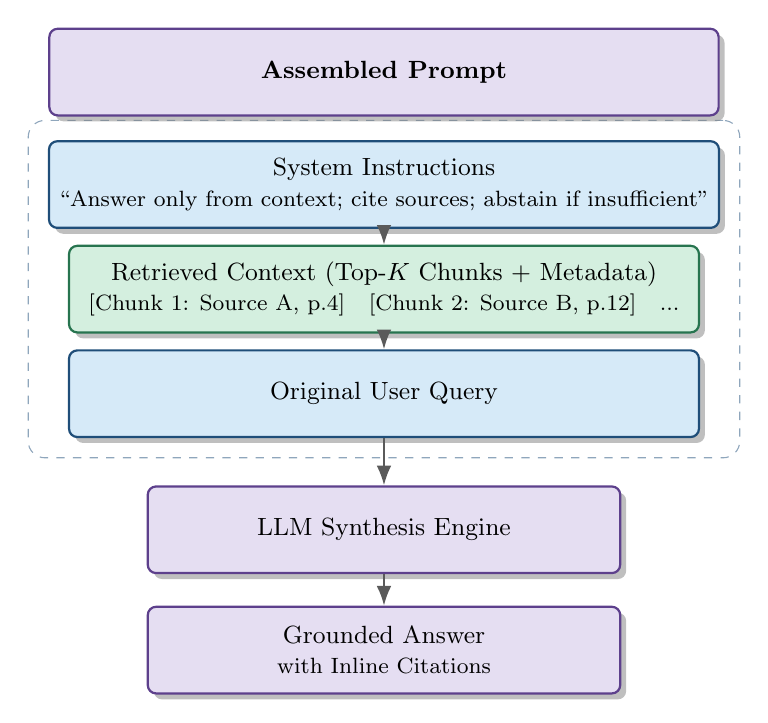
\begin{tikzpicture}[node distance=0.5cm]

\node[genblock, minimum width=8.5cm] (prompt) {\textbf{Assembled Prompt}};
\node[block, below=0.3cm of prompt, minimum width=8cm, fill=raglight] (sys) {System Instructions \\ \footnotesize ``Answer only from context; cite sources; abstain if insufficient''};
\node[storeblock, below=0.2cm of sys, minimum width=8cm] (ctx) {Retrieved Context (Top-$K$ Chunks + Metadata) \\ \footnotesize [Chunk 1: Source A, p.4] \ \ [Chunk 2: Source B, p.12] \ \ ...};
\node[block, below=0.2cm of ctx, minimum width=8cm, fill=raglight] (uq) {Original User Query};

\node[genblock, below=0.6cm of uq, minimum width=6cm] (llm) {LLM Synthesis Engine};
\node[genblock, below=0.4cm of llm, minimum width=6cm, fill=raglightpurple] (out) {Grounded Answer \\ \footnotesize with Inline Citations};

\draw[arrowflow] (sys) -- (ctx);
\draw[arrowflow] (ctx) -- (uq);
\draw[arrowflow] (uq.south) -- ++(0,-0.15) -| (llm.north);
\draw[arrowflow] (llm) -- (out);

\begin{scope}[on background layer]
\node[fit=(sys)(ctx)(uq), inner sep=0.25cm, rounded corners=6pt, draw=ragblue!50, dashed] {};
\end{scope}

\end{tikzpicture}
\caption{Anatomy of the final augmented prompt and the synthesis step: system instructions, retrieved context with provenance metadata, and the original query are assembled and passed to the LLM, which produces a grounded, citable answer.}
\label{fig:prompt-injection}
\end{figure}

\newpage

% =========================================================
\section{Visual Diagrams: End-to-End Data Flow}
\sectionrule

This section consolidates the pipeline into a single, detailed, vertically-oriented diagram tracing a concrete unit of data --- a document and a user query --- through every architectural stage discussed above.

\begin{figure}[htbp]
\centering
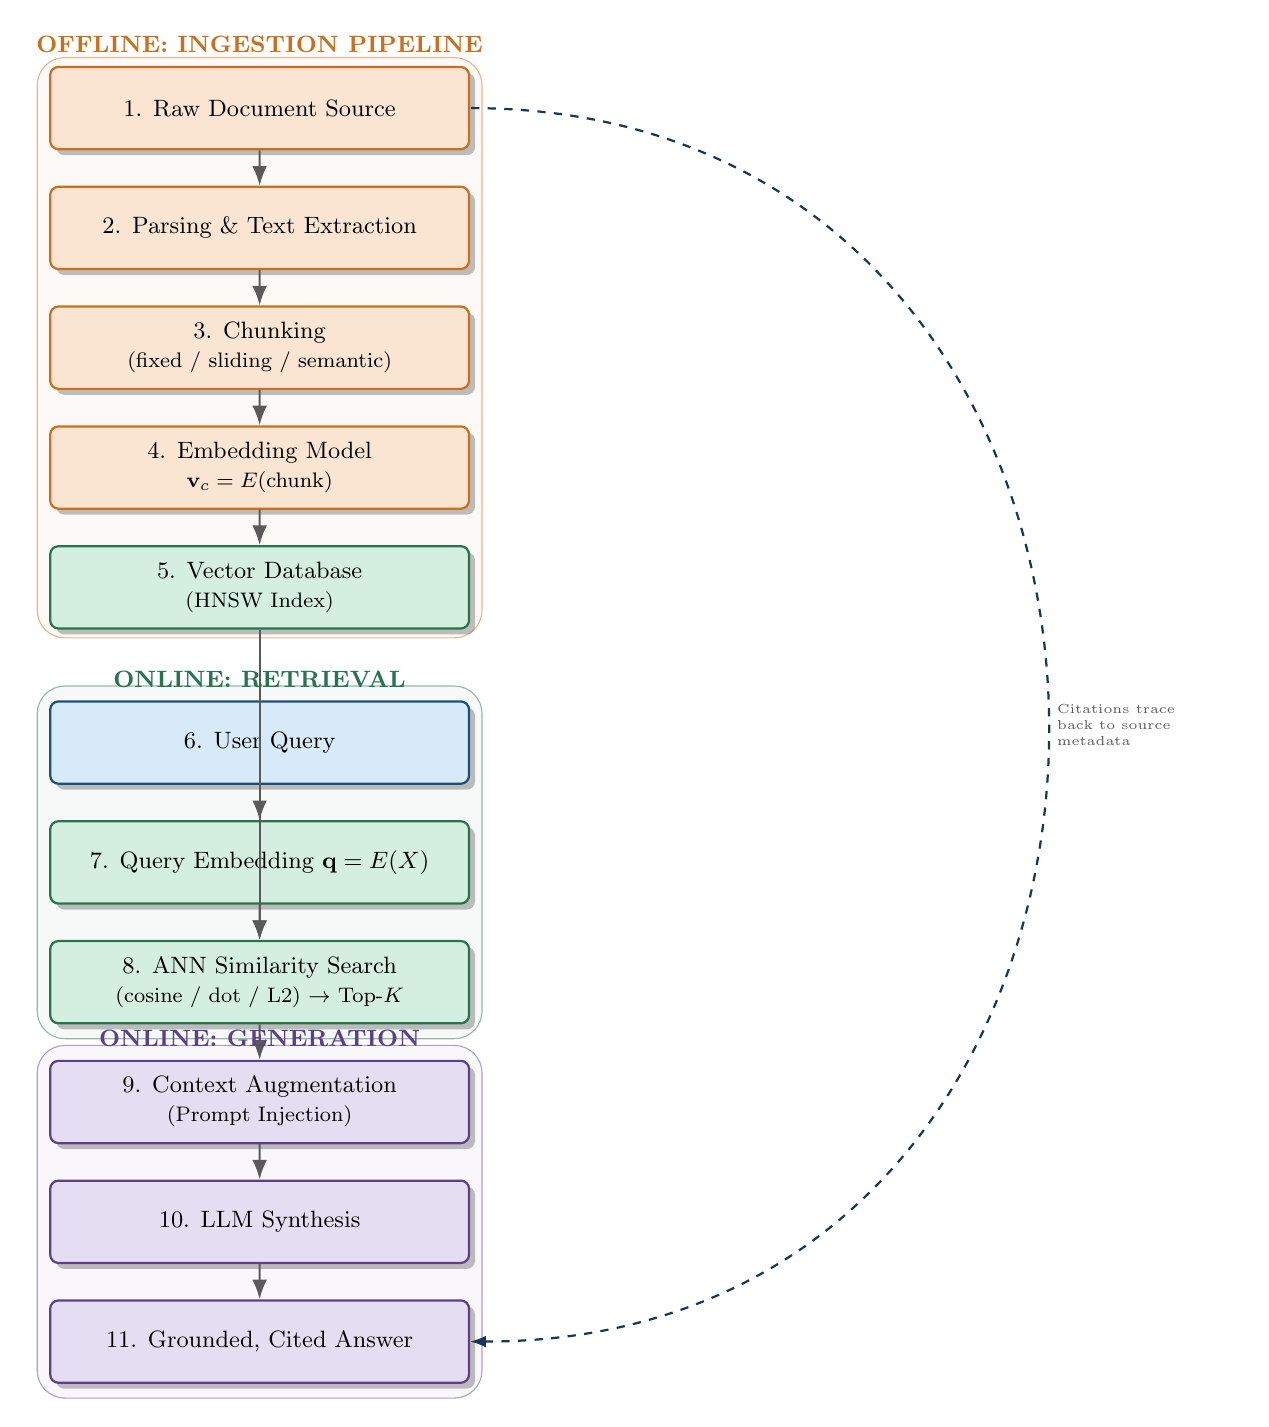
\begin{tikzpicture}[node distance=0.45cm, scale=0.95, every node/.style={scale=0.95}]

% -------- OFFLINE INGESTION TRACK (left) --------
\node[ingestblock, minimum width=5.6cm] (n1) {1. Raw Document Source};
\node[ingestblock, below=of n1, minimum width=5.6cm] (n2) {2. Parsing \& Text Extraction};
\node[ingestblock, below=of n2, minimum width=5.6cm] (n3) {3. Chunking \\ \footnotesize (fixed / sliding / semantic)};
\node[ingestblock, below=of n3, minimum width=5.6cm] (n4) {4. Embedding Model \\ \footnotesize $\mathbf{v}_c = E(\text{chunk})$};
\node[storeblock, below=of n4, minimum width=5.6cm] (n5) {5. Vector Database \\ \footnotesize (HNSW Index)};

\foreach \a/\b in {n1/n2,n2/n3,n3/n4,n4/n5}
  \draw[arrowflow] (\a) -- (\b);

\node[phase, above=0.05cm of n1, text=ragorange] {OFFLINE: INGESTION PIPELINE};

% -------- ONLINE RETRIEVAL + GENERATION TRACK (continuing down) --------
\node[block, below=0.9cm of n5, minimum width=5.6cm, fill=raglight] (n6) {6. User Query};
\node[storeblock, below=of n6, minimum width=5.6cm] (n7) {7. Query Embedding $\mathbf{q}=E(X)$};
\node[storeblock, below=of n7, minimum width=5.6cm] (n8) {8. ANN Similarity Search \\ \footnotesize (cosine / dot / L2) $\to$ Top-$K$};
\node[genblock, below=of n8, minimum width=5.6cm] (n9) {9. Context Augmentation \\ \footnotesize (Prompt Injection)};
\node[genblock, below=of n9, minimum width=5.6cm] (n10) {10. LLM Synthesis};
\node[genblock, below=of n10, minimum width=5.6cm, fill=raglightpurple] (n11) {11. Grounded, Cited Answer};

\foreach \a/\b in {n6/n7,n7/n8,n8/n9,n9/n10,n10/n11}
  \draw[arrowflow] (\a) -- (\b);

\draw[arrowflow] (n5) -- (n8);
\node[phase, above=0.05cm of n6, text=raggreen] {ONLINE: RETRIEVAL};
\node[phase, above=0.05cm of n9, text=ragpurple] {ONLINE: GENERATION};

% Feedback / citation loop back to source metadata
\draw[dataflow, {Latex[length=2mm]}-] (n11.east) to[out=0,in=0,looseness=1.6] node[right, font=\tiny, text=raggray, align=left] {Citations trace\\ back to source\\ metadata} (n1.east);

\begin{scope}[on background layer]
\node[fit=(n1)(n5), inner sep=0.3cm, rounded corners=10pt, draw=ragorange!50, fill=ragorange!4] {};
\node[fit=(n6)(n8), inner sep=0.3cm, rounded corners=10pt, draw=raggreen!50, fill=raggreen!4] {};
\node[fit=(n9)(n11), inner sep=0.3cm, rounded corners=10pt, draw=ragpurple!50, fill=ragpurple!4] {};
\end{scope}

\end{tikzpicture}
\caption{Consolidated vertical end-to-end RAG architecture diagram. The offline ingestion pipeline (top, executed once or periodically) populates the vector database that the online retrieval-and-generation pipeline (bottom, executed per user query) depends upon. The dashed feedback loop indicates that the final answer's citations trace back to the original source metadata captured during ingestion.}
\label{fig:full-vertical-pipeline}
\end{figure}

\newpage

% =========================================================
\section{Synthesis: Design Trade-offs and Closing Remarks}
\sectionrule

\subsection{Summary of Key Design Levers}

\begin{center}
\begin{tabular}{@{}p{3.6cm}p{5.6cm}p{5.2cm}@{}}
\toprule
\textbf{Design Lever} & \textbf{Trade-off} & \textbf{Impacted Stage} \\
\midrule
Chunk size / overlap & Precision vs.\ context sufficiency & Ingestion (Chunking) \\
Embedding model choice & Semantic fidelity vs.\ inference cost & Ingestion (Embedding) \\
ANN index parameters & Recall vs.\ query latency & Storage \& Retrieval \\
Similarity metric & Alignment with embedding geometry & Storage \& Retrieval \\
Top-$K$ value & Coverage vs.\ context-window budget & Retrieval \\
Re-ranking & Precision gain vs.\ added latency & Retrieval \\
Prompt structure & Faithfulness vs.\ verbosity & Prompt Injection \& Generation \\
\bottomrule
\end{tabular}
\end{center}

\subsection{Closing Remarks}

Retrieval-Augmented Generation reframes the LLM not as an omniscient oracle, but as a powerful \textbf{reasoning and synthesis engine} operating over an explicitly supplied, verifiable, and continuously updatable body of evidence. By decomposing the system into an ingestion pipeline that structures raw knowledge, a retrieval subsystem that locates relevant evidence with geometric similarity search, and a generation subsystem that synthesizes grounded natural language, RAG architectures directly target the core weaknesses of parametric-only language models: hallucination, staleness, and opacity. Every design decision along this pipeline --- from how a document is chunked to which similarity metric indexes its vectors --- propagates forward and ultimately shapes the faithfulness and utility of the final generated answer, making end-to-end architectural literacy, rather than any single component in isolation, the true foundation of effective RAG system design.

% =========================================================
\newpage
\section{References}
\sectionrule
\bibliography{references}

\end{document}